\documentclass[11pt]{beamer}
\usetheme{JuanLesPins}
\usepackage[utf8]{inputenc}
\usepackage[spanish]{babel}
\usepackage{amsmath}
\usepackage{amsfonts}
\usepackage{amssymb}
\usepackage[tikz]{}
\usepackage{graphicx}
\usepackage{adjustbox}
\usepackage{array}
\spanishdecimal{.}
\author{M. en E. Sergio Nava}
\title{Variables Aleatorias Discretas}
%\setbeamercovered{transparent} 
%\setbeamertemplate{navigation symbols}{} 
%\logo{} 
%\institute{} 
\date{Viernes 5 de octubre de 2018} 
%\subject{} 

\AtBeginSection[]  % The commands within the following {} will be executed at the start of each section.
{
\begin{frame} % Within each "frame" there will be one or more "slides."  
\frametitle{Presentation Outline} % This is the title of the outline.
\tableofcontents[currentsection]  % This will display the table of contents and highlight the current section.
\end{frame}
} % Do not include the preceding set of commands if you prefer not to have a recurring outline displayed during your presentation.


\begin{document}

\begin{frame}
\titlepage
\end{frame}



\section{Distribución Uniforme Discreta}

\begin{frame}{Uniforme discreta}
\begin{enumerate}
\item Una variable aleatoria que tiene $n$ posibles resultados
\item Los n resultados posibles son igualmente probables
\end{enumerate}
Si la distribución toma los valores reales $x_{1},x_{2}\ldots x_{n}$, su función de probabilidad es
$$ P(X=x_{i})={\frac {1}{n}}\,$$
y su función de distribución la función escalonada
$$F(x)={\frac {1}{n}}\sum _{i}1_{(-\infty ,x]}(x_{i}) ,$$
\end{frame}
\begin{frame}
Su media es

$$E(X)=\mu ={\frac {1}{n}}\sum _{i}^{n}x_{i},$$

y su varianza

$$Var(X)=\sigma ^{2}={\frac {1}{n}}\sum _{i=1}^{n}(x_{i}-\mu )^{2}={\frac {1}{n}}\sum _{i=1}^{n}(x_{i}^{2})-\mu ^{2}\,$$
\end{frame}
\begin{frame}{Ejemplo de v.a. Uniforme Discreta}
Consideremos el ejemplo de tirar un dado.  Hay n=6 valores posibles de la variable aleatoria, son x=1,2,3,4,5,6 por consiguiente, la función de probabilidad para esta variable aleatoria es  
\begin{center}
$P(x)=1/6$\hspace{20pt}   $x=1,2,3,4,5,6$ \hspace{20pt}  $F(x)= \lfloor x \rfloor /6$

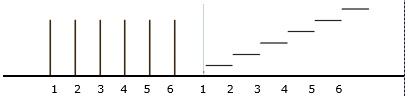
\includegraphics[scale=0.8]{imagenes/prob46.jpg} 
\end{center}
$$E(X)=3.5 \hspace{20pt} Var(X)=\frac{35}{12}$$ 
\end{frame}

\begin{frame}{Ejercicio}
Considere la ruleta de un casino con n\'umeros del 0 al 36. 

Determine:

\begin{enumerate}
  \item Probabilidad de que caiga un 20
  \item Probabilidad de que caiga un n\'umero entre 20 y 28
\end{enumerate}
\end{frame}

\section{Experimento y Variable Aleatoria Bernoulli}


\begin{frame}{Bernoulli}
\begin{enumerate}
\item Una v.a. que tiene dos posibles resultados, a uno le llamamos éxito y  le asignamos el valor de $1$ y al otro fracaso y le asignamos $0$.
\item La probabilidad de éxito se representa por $p$, no cambia de un intento o ensayo a otro.
\item Por lo tanto, la probabilidad de fracaso, representada por $q=1-p$ tampoco cambia.
\item Los intentos o ensayos son independientes
\end{enumerate}
\end{frame}
\begin{frame}{Ejemplo Bernoulli}
\begin{itemize}
\item Un volado es una v.a. Bernoulli,   
\item si la moneda no esta cargada, entonces la probabilidad de éxito es  $p=\frac{1}{2}$.
\end{itemize}
\begin{center}
{\large \textbf{¿Se cumplen las condiciones de una variable aleatoria Bernoulli?}}
\end{center}
\end{frame}
\begin{frame}{Bernoulli}
El valor esperado y la varianza de una variable aleatoria Bernoulli dada p son:
\begin{center}
$E(X)=p \hspace{2cm} Var(X)=p q$
\end{center}
Para el ejemplo del lanzamiento de una moneda 
\begin{center}
$E(x)=1/2 \hspace{2cm} Var(X)=1/4$
\end{center}
\end{frame}
\begin{frame}{Ejemplos de v.a. Bernoulli}
Dé tres ejemplos de v.a. Bernoulli que no sean \textit{el lanzamiento de una moneda}.
Y calcule su valor esperado y varianza

\end{frame}


\begin{frame}{Ejercicio}
Considere la ruleta de un casino con n\'umeros del 0 al 36. Considere éxito que caiga el número elegido

\bigskip
Determine:

\begin{enumerate}
  \item $p$
  \item $E(X)$
  \item $Var(X)$
\end{enumerate}
\end{frame}

\section{Distribución Binomial}


\begin{frame}{Binomial}
Un experimento binomial tiene las siguientes características:
\begin{enumerate}
\item El experimento consiste de $n$ ensayos idénticos
\item Cada ensayo produce uno de dos resultados posibles (éxito o fracaso)
\item La probabilidad de éxito en un sólo ensayo es $p$, y es constante para todos los ensayos (la probabilidad de fracaso es $q = 1 - p$).
\item Los ensayos son independientes entre si
\item El experimentador está interesado en la variable $X$, que representa el número de aciertos observados en los $n$ ensayos.

\end{enumerate}
\end{frame}
\begin{frame}{Binomial}
Equivalentemente un experimento binomial tiene las siguientes características:
\begin{enumerate}
\item El experimento consiste de n ensayos Bernoulli, con probabilidad de éxito $p$
\item Los ensayos son independientes entre si
\item El experimentador está interesado en la variable $X$, que representa el número de aciertos observados en los $n$ ensayos.
\end{enumerate}
\end{frame}
\begin{frame}{Ejemplo de lanzar una moneda}
\begin{itemize}
\item Para $n = 1$ ensayo, como se tienen dos puntos muestrales, $E_1$ representado por A=águila (éxito), y $E_2$ representado por S=sol (fracaso), con probabilidades $p$ y $q$ respectivamente.
\item Dado que $X$ es el número de aciertos en $n$ los posibles resultados en un ensayo son $X = 1$ cuando ocurre águila y $X = 0$ cuando es sol.
\end{itemize}
\end{frame}
\begin{frame}{Ejemplo de lanzar dos moneda}
Para n = 2 ensayos, la probabilidad de los eventos se calcula por la ley multiplicativa de la probabilidad, esto es:
\begin{center}
\begin{tabular}{ll}
$P(E_{1})=P(AA)=P(A)P(A)=p^{2}$\hspace{2cm}&$x=2$ \\ 
$P(E_{2})=P(AS)=P(A)P(S)=pq$&$x=1$ \\
$P(E_{3})=P(SA)=P(S)P(A)=pq$&$x=1$ \\
$P(E_{4})=P(SS)=P(S)P(S)=q^{2}$&$x=0$ \\

\end{tabular}
\end{center}
\end{frame}
\begin{frame}{Ejemplo de lanzar dos moneda}
\begin{itemize}
\item De esta forma, las probabilidades se representan como:
\begin{center}
\begin{tabular}{l|l}
\textbf{x}&\textbf{p(x)} \\ \hline
2&$p^{2}$ \\
1&2pq \\
0&$q^{2}$ \\
\end{tabular}
\end{center}
\item La distribución de probabilidad se obtiene de la expansión de $(p + q)^{n}$; que para $n = 2$ es:
$$\sum_{x=0}^{2}p(x)=(p+q)^{2}=p^{2}+2pq+q^{2}=1$$
\end{itemize}
\end{frame}
\begin{frame}{Distribución de Probabilidad Binomial}
\begin{itemize}
\item La distribución de probabilidad binomial en forma general se define como:
$$p(x;n,p)=p(x)=\binom{n}{x}\cdot p^{x}\cdot q^{n-x}=\frac{n!}{x!(n-x)!}\cdot p^{x}\cdot q^{n-x}$$
donde $x$ toma los valores $0, 1, 2, \ldots , n$.
\item La función de distribución acumulada binomial es:
$$F(x;n,p)=P(X \le x)=\sum_{i \le x}\binom{n}{i}p^{i}\cdot q^{n-i}$$
\end{itemize}
\end{frame}
\begin{frame}{Distribución de Probabilidad Binomial (Triangulo de Pascal)}
\begin{center}
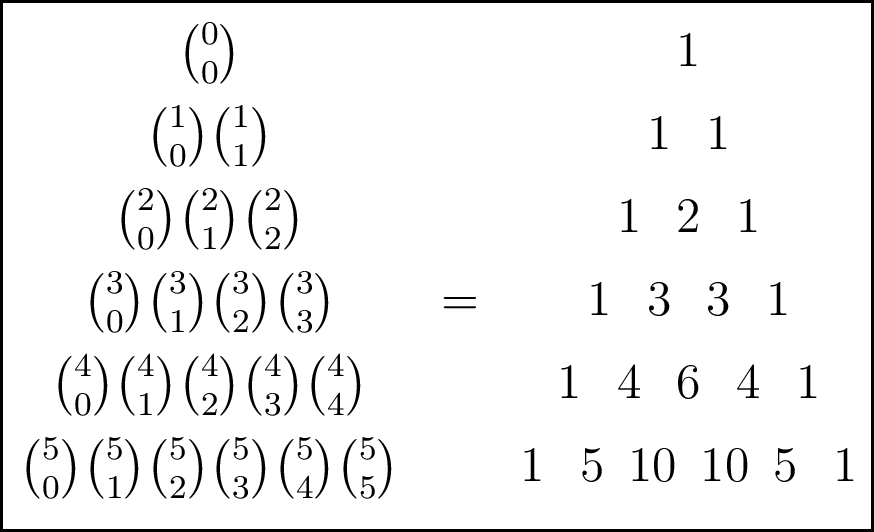
\includegraphics[scale=0.3]{ilustraciones/7NttW.png} 
\end{center}
\end{frame}
\begin{frame}{Distribución de Probabilidad Binomial}
\begin{center}
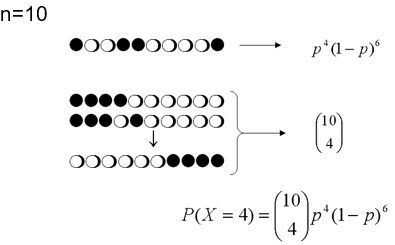
\includegraphics[scale=0.8]{imagenes/prob47.jpg} 
\end{center}
\end{frame}
\begin{frame}{Binomial}
El valor esperado y la varianza de una variable aleatoria binomial dados $n$ y $p$ son:
$$E(X)=n\cdot p \hspace{2cm} Var(X)=n\cdot p\cdot q$$
\end{frame}
\begin{frame}{Distribución de Probabilidad Binomial}
\begin{center}
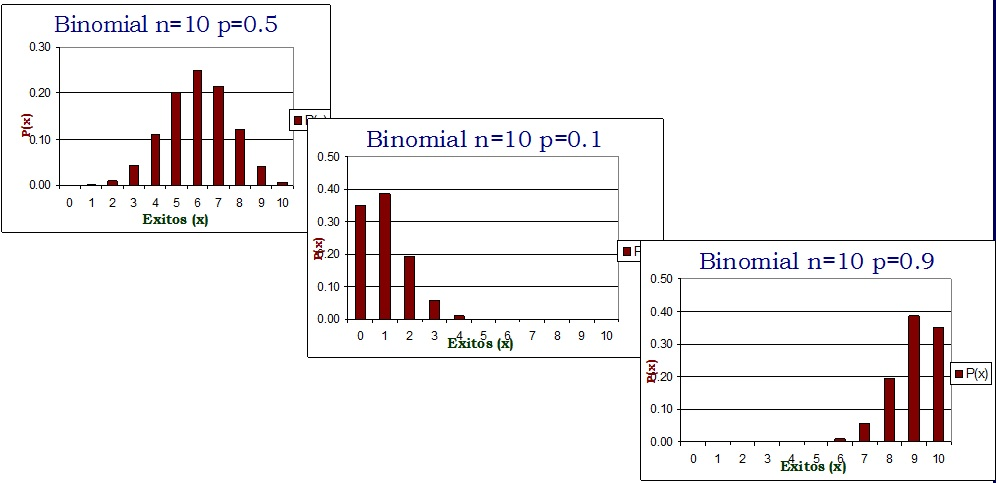
\includegraphics[scale=0.4]{imagenes/prob48.jpg} 
\end{center}
\end{frame}
\begin{frame}{Ventas por teléfono}
Una compañía de ventas por teléfono, indica que de cada 11 llamadas realizadas, 3 resultan en ventas.
Con base en esto, la compañía desea saber:
\begin{enumerate}
\item ¿cuál es la probabilidad de que de 10 llamadas que recibas 6 resulten en ventas?.
\item ¿cuál es la probabilidad de que de 10 llamadas ninguna sea venta?
\item ¿qué probabilidad tiene de realizar a lo más 5 ventas en 10 llamadas?
\end{enumerate}
\end{frame}


\begin{frame}{Ejercicio}
Considere la ruleta de un casino con n\'umeros del 0 al 36. Considere éxito que caiga el número elegido. Suponga que decide jugar 15 veces. 

\bigskip
Determine:

\begin{enumerate}
  \item $p$
  \item La expresión para calcular $P(x)$
  \item $P(X  < 3)$
  \item $E(X)$
  \item $Var(X)$
\end{enumerate}
\end{frame}


\section{Distribución Geométrica}


\begin{frame}{Geométrica}
Sea $X$ la variable que representa el número de fracasos antes de obtener el primer éxito en experimentos Bernoulli independientes, cada uno con probabilidad $p$.
\end{frame}

\begin{frame}{Geométrica}
\begin{itemize}
\item La distribución de probabilidad geométrica se define como:
$$p(x;p)=(1-p)^x \cdot p=q^x \cdot p$$ 
donde $x$ toma los valores $0,1,2,\ldots $
\item La función de distribución acumulada geométrica es :
$$F(x;p)=P(X \le x)= \sum_{i=0}^{x}q^i \cdot p$$
\end{itemize}
\end{frame}


\begin{frame}
\newpage
\begin{Large}
\begin{flushleft}
\textbf{Geom\'etrica}
\end{flushleft}
\end{Large}
El valor esperado y la varianza de una variable aleatoria geom\'etrica dada por $p$ son:
$$E\left( X \right) =\frac { \left( 1-p \right)  }{ p } $$
$$Var\left( X \right) =\frac { \left( 1-p \right)  }{ { p }^{ 2 } }$$
\end{frame}

\begin{frame}{Geométrica}

\begin{figure}[hbtp]
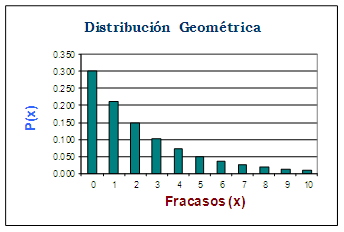
\includegraphics[scale=0.5]{ilustraciones/1.png}

%ilustracion1% 
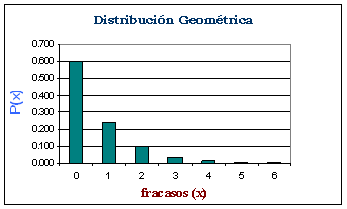
\includegraphics[scale=0.5]{ilustraciones/2.png} 
%ilustracion2% 
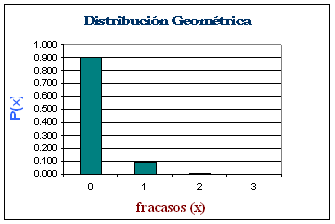
\includegraphics[scale=0.5]{ilustraciones/3.png} 
%ilustracion3%
\end{figure}\end{frame}

\begin{frame}{Geom\'etrica}
\begin{itemize}
\item Una característica de la distribución geométrica que es importante destacar, es lo que se conoce como "falta de memoria". Se dice que la distribución geométrica "no tiene memoria".

\item La distribución geométrica no es afectada por los resultados anteriores.

\item Es decir, no importa desde cuándo empecemos a contar, siempre la probabilidad de las distintas cantidades de intentos hasta alcanzar un éxito estará distribuida de la misma forma.
\end{itemize}
\end{frame}

\begin{frame}{Geom\'etrica}

No importa si empezamos a contar justo después de un éxito, o después de una racha de 30 fracasos.

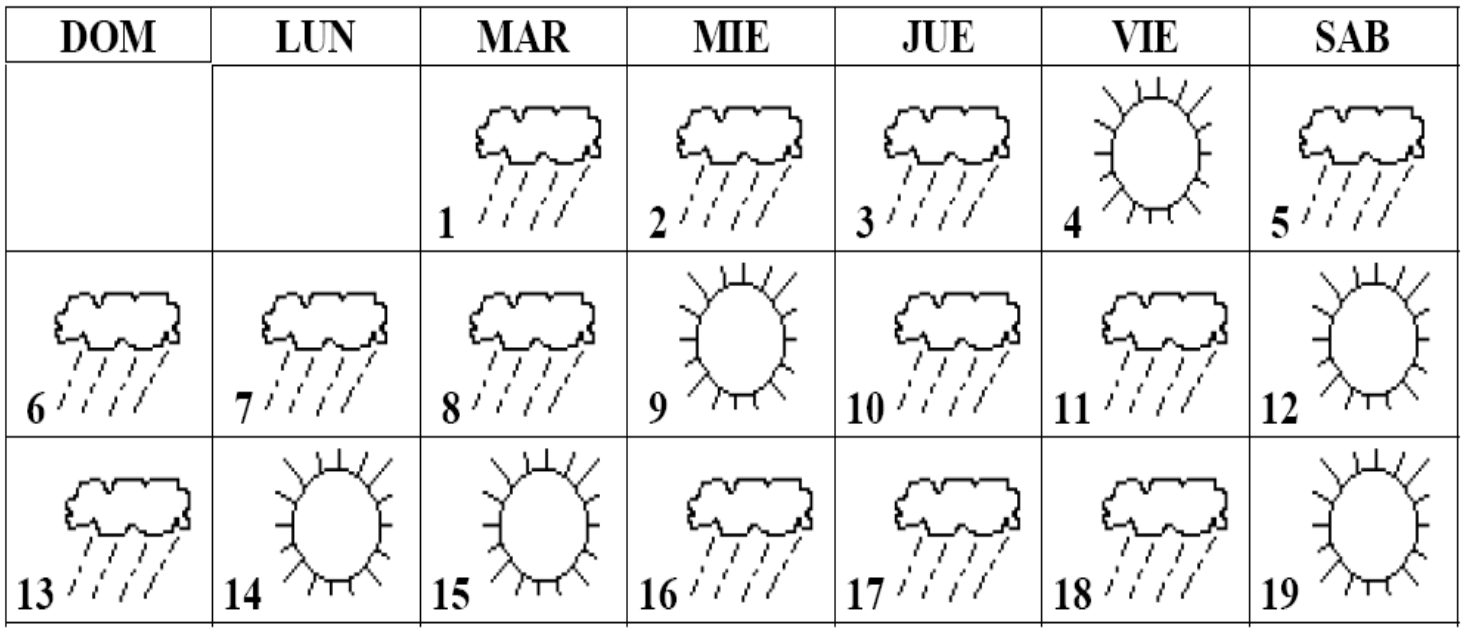
\includegraphics[scale=0.4]{ilustraciones/4.png} 
%ilustracion4%
\end{frame}

\begin{frame}{Ejemplo}

Necesitamos establecer una conexión. Cada vez que intentamos conectarnos, tenemos una probabilidad de 0.2 de lograr establecer la conexión.
\begin{enumerate}
\item ¿Cuál es la probabilidad de que logremos conectarnos en menos de 4 intentos?

\item  ¿Cuántas veces es de esperar que tengamos que intentar conectarnos hasta lograrlo?

\item Si cada intento nos lleva 20 segundos y además perdemos 10 segundos entre intento e intento para dejar todo listo para volver a intentar, ¿cuánto tiempo se espera que nos lleve el proceso de conectarnos?
\end{enumerate}
\end{frame}


\begin{frame}{Ejercicio}
Considere la ruleta de un casino con n\'umeros del 0 al 36. Considere éxito que caiga el número elegido.  Es decir, se jugará hasta ganar por primer vez. 

\bigskip
Determine:

\begin{enumerate}
  \item $p$
  \item La expresión para calcular $P(x)$
  \item $P(X  < 3)$
  \item $E(X)$
  \item $Var(X)$
\end{enumerate}
\end{frame}


\section{Distribución Binomial Negativa}



\begin{frame}{Binomial negativa}
\begin{itemize}
\item Se utiliza en experimentos bernoulli en los cuales interesa el número de fracasos antes de alcanzar $k$ éxitos.

\item  Esto es un experimento bernoulli en donde la probabilidad de éxito en cada ensayo es $p$

\end{itemize}
\end{frame}

\begin{frame}{Binomial negativa}
La distribución de probabilidad binomial negativa se define por:
$$p(x;k,p)=\binom{k+x-1}{x} \cdot p^k \cdot (1-p)^x \mbox{ para }x=0,1,2, \ldots$$ 
$k=$número de éxitos \\
$x=$número de fracasos\\
$p=$probabilidad de éxito
\end{frame}


\begin{frame}{Binomial negativa}
El valor esperado y la varianza de una variable binomial negativa es:
$$E(X)=\frac{k \cdot (1-p)}{p}$$
$$Var(X)=\frac{k \cdot (1-p)}{p^2}$$
\end{frame}

\begin{frame}{Binomial negativa: Gráfico Función de Probabilidad}
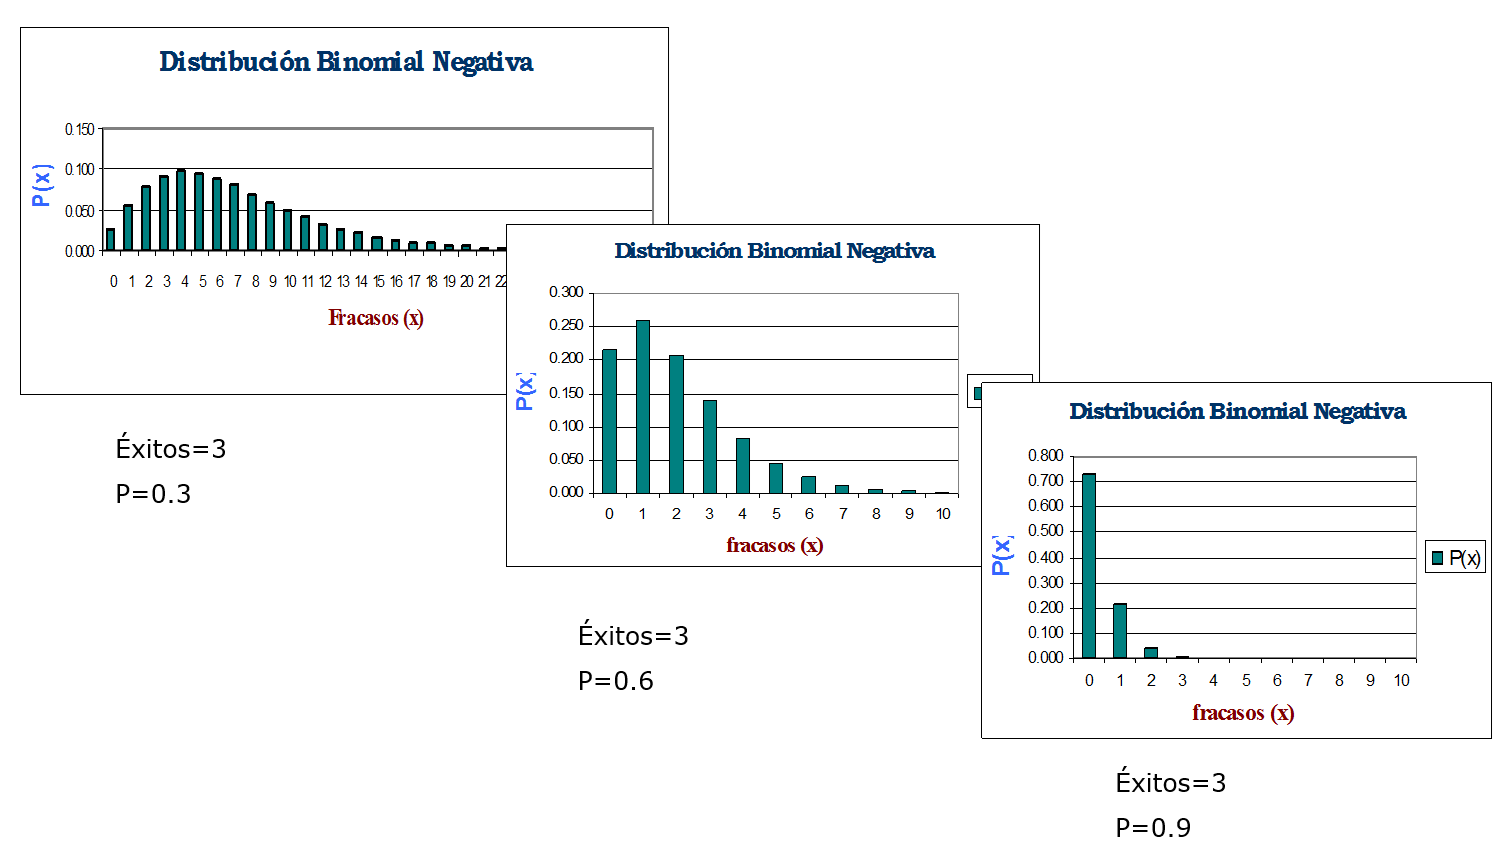
\includegraphics[scale=0.4]{ilustraciones/BN.png} 
\end{frame}

\begin{frame}{Binomial negativa: Ejemplo de personas con perros}
La probabilidad de que una persona, que vive en cierta ciudad, tenga un perro se estima en 0.3. Encuentre la probabilidad de que la décima persona entrevistada al azar en esta ciudad sea la tercera que tiene un perro.
$$p(7;3,0.3)=\binom{9}{7} (.3)^3 (.7)^7 =0.080$$
¿En promedio cuantas personas sin perro necesito entrevistar para encontrar a tres que tengan perro?
$$E(X)=\frac{k \cdot (1-p)}{p}=\frac{3 \cdot (1-.3)}{.3}=7$$
\end{frame}

\begin{frame}{Ejercicio}
Un pediatra desea reclutar cinco parejas, cada una de las cuales espera a su primer hijo, para participar en un nuevo régimen de alumbramiento natural. Sea $p=P($una pareja seleccionada
al azar está de acuerdo en participar$)$. Si $p=0.2$, ¿cuál es la probabilidad de que $15$ parejas tengan que ser entrevistadas antes de encontrar cinco que estén de acuerdo en participar?
Es decir, $E=\{$está de acuerdo en participar$\}$, ¿cuál es la probabilidad de que ocurran $10$ fallas antes del quinto éxito?

\bigskip
Determine además:
			
\begin{enumerate}
  \item $P(X)$
  \item $E(X)$
  \item $Var(X)$
\end{enumerate}

\end{frame}


\section{Distribución Hipergeométrica}


\begin{frame}{Hipergeom\'etrica}

\begin{itemize}
\item Esta distribución se utiliza cuando se estudian fen\'omenos con caracter\'isticas de experimento binomial. 

\item La distribuci\'on binomial supone que la extracci\'on de los resultados del ensayo son \textit{con reemplazo}, por lo  que la probabilidad es constante de ensayo a ensayo. 

\item En la pr\'actica es m\'as com\'un que la extracci\'on de los resultados del ensayo sea \textit{sin reemplazo} 
\end{itemize}
\end{frame}

\begin{frame}{Hipergeom\'etrica notaci\'on}

En \'este caso, se define la siguiente notaci\'on:
\\ \bigskip
$N =$ n\'umero de elementos en la poblaci\'on

$k =$ n\'umero de elementos en la poblaci\'on que se consideran \'exitos (es decir que poseen la caracter\'istica de inter\'es)

$n =$ n\'umero de elementos en la muestra tomados de los $N$ elementos en la poblaci\'on

$x =$ n\'umero de \'exitos en la muestra
\begin{flushright}
 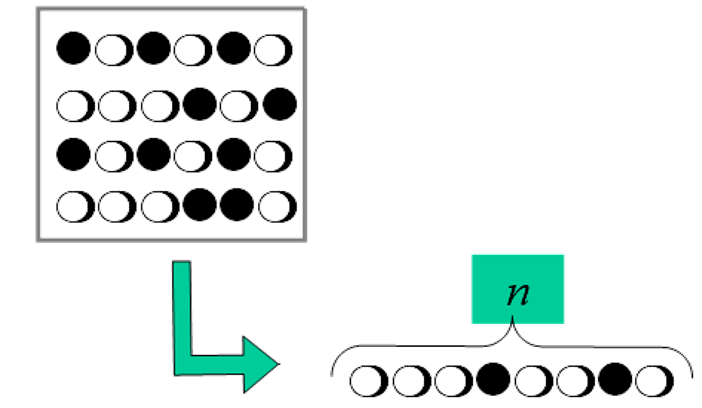
\includegraphics[scale=0.4]{ilustraciones/urnaH.png} 
 \end{flushright}
\end{frame}

\begin{frame}{Hipergeom\'etrica}
La distribución de probabilidad Hipergeométrica se obtiene por:


$$p\left( x;N,n,k \right) =\frac { \binom{k}{x} \cdot \binom{N-k}{n-x}}{\binom{N}{n}} $$
para

$x=0,1,\ldots, n,\quad si\quad n<k$

$x=0,1,\ldots , k,\quad si\quad n\ge k$
\end{frame}

\begin{frame}{Hipergeom\'etrica}
El valor esperado y la varianza de una variable hipergeométrica es:

$$E\left( x \right) =\frac { n\cdot k }{ N } $$

$$Var\left( x \right) =\frac { n\cdot k\cdot \left( N-k \right)  }{ { N }^{ 2 } } \cdot \frac { N-n }{ N-1 } $$
\end{frame}

\begin{frame}{Hipergeom\'etrica}
Muestras con $n=10$
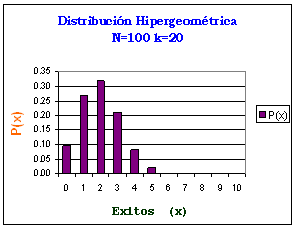
\includegraphics[scale=0.5]{ilustraciones/5.png} 
%ilustracion5% 
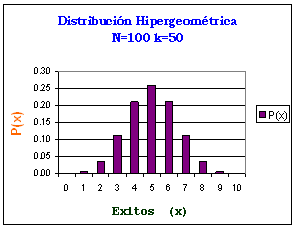
\includegraphics[scale=0.5]{ilustraciones/6.png} 
%ilustracion6%
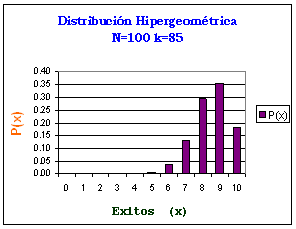
\includegraphics[scale=0.5]{ilustraciones/7.png} 
%ilustracion7%
\end{frame}

\begin{frame}{Ejemplo de pol\'iticos}

Supóngase que se tienen 20 representantes de cierto estado en una convención política nacional, de los cuales 15 apoyan al candidato A y 5 apoyan al candidato B. Si se seleccionan aleatoriamente a 4 representantes sin reemplazo, 
\begin{enumerate}
\item ¿Cuál es la probabilidad de que entre estos 4, por lo menos 2 apoyen al candidato A?

\item ¿Cuál es la probabilidad de que entre estos 4, ninguno apoye al candidato A?

\item ¿Cuál es la probabilidad de que entre estos 4, ninguno apoye al candidato B?
\end{enumerate}
\end{frame}

\begin{frame}{Hipergeom\'etrica}

¿Qué otro ejemplo hemos visto de distribuci\'on Hipergeom\'etrica?
\end{frame}


\begin{frame}{Ejercicio}
Durante un periodo particular una oficina de tecnología de la información de una universidad recibió $20$ solicitudes de servicio de problemas con impresoras, de las cuales $8$ eran impresoras
láser y $12$ eran modelos de inyección de tinta. Se tiene que seleccionar una muestra de $5$ de estas solicitudes de servicio completamente al azar, de modo que cualquier subconjunto
de tamaño $5$ tenga la misma probabilidad de ser seleccionado como cualquier otro subconjunto (piense en escribir los números $1, 2,  \ldots , 20$  en $20$ papelitos idénticos, mezclarlos
y seleccionar $5$ de ellos). ¿Cuál es entonces la probabilidad de que exactamente $x$ $(x= 0, 1, 2, 3, 4$ o $5)$ de las solicitudes de servicio fueran para impresoras de inyección de tinta?
\bigskip
Determine :
\begin{enumerate}
  \item $P(X=2)$
  \item $E(X)$
  \item $Var(X)$
\end{enumerate}

\end{frame}


\section{Distribución Poisson}


\begin{frame}{Poisson}
La variable aleatoria Poisson representa el número de eventos independientes que ocurren en una unidad de espacio (tiempo, distancia, área, volumen, etc.).

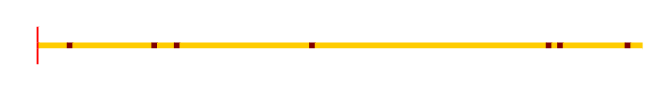
\includegraphics[scale=0.5]{ilustraciones/puntosP.png} 
\end{frame}

\begin{frame}{Poisson}

Distribución de probabilidad Poisson:

$$p\left( x;\lambda  \right) =\frac { { e }^{ -\lambda  }\cdot { \lambda  }^{ x } }{ x! }\hspace{1cm} \mbox{ para } x=0,1,2,...;\lambda      >0$$

donde $\lambda$ es el parámetro de la distribución Poisson, que representa el número promedio de ocurrencias del evento aleatorio por unidad de espacio (tiempo, área, volumen o distancia).
\end{frame}

\begin{frame}{Poisson}
El valor esperado y la varianza de una variable Poisson es:




$$E\left[ X \right] =\lambda$$
$$Var\left[ X \right] =\lambda$$

\end{frame}

\begin{frame}{Poisson}
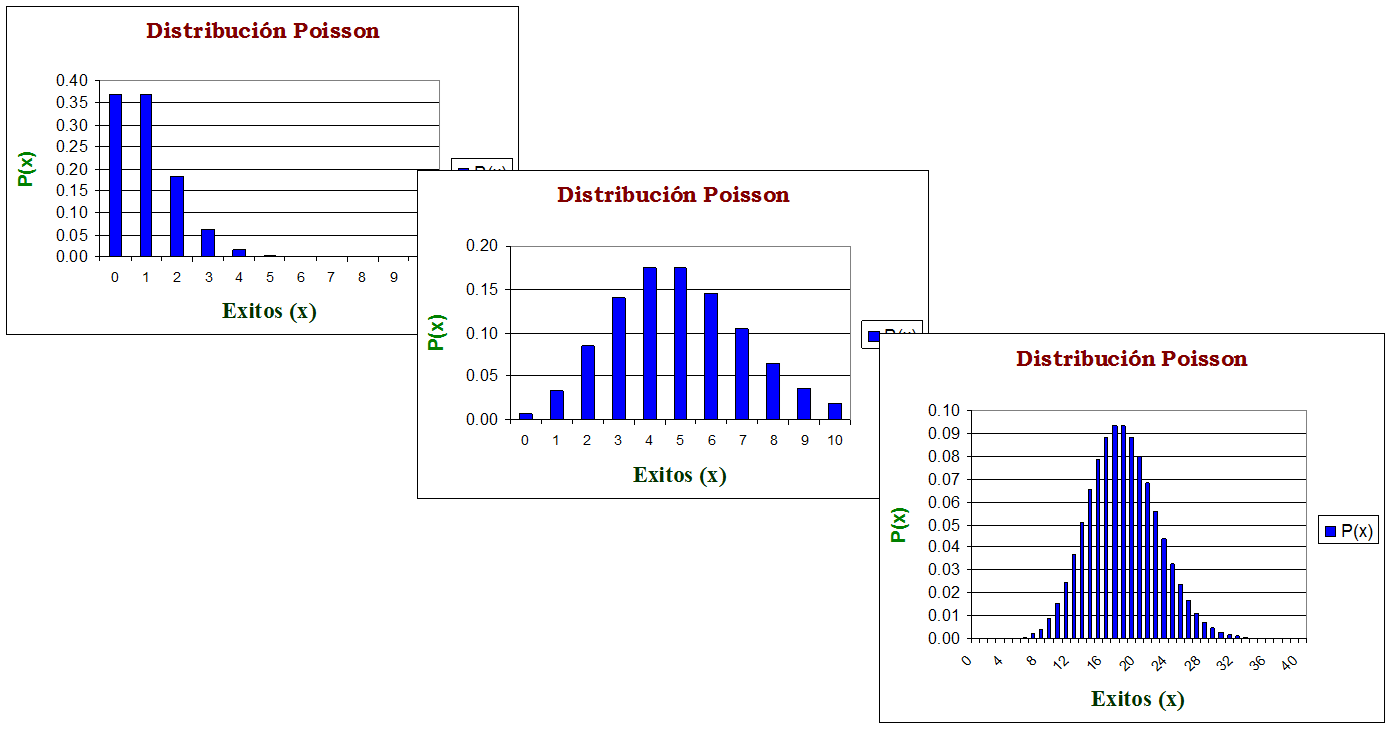
\includegraphics[scale=0.5]{ilustraciones/Poisson.png} 
\end{frame}

\begin{frame}{Poisson: Ejemplo  Infracciones}

El número de infracciones expedidas por el lector de un parquímetro, por violaciones de estacionamiento, puede modelarse mediante un proceso de Poisson con una tasa de cinco infracciones por hora.
\begin{enumerate}
\item¿Cuál es la probabilidad de que exactamente cinco infracciones se expidan durante una hora particular?

\item ¿Cuál es la probabilidad de que por lo menos tres infracciones se expidan durante una hora particular?

\item ¿Cuántas infracciones se espera expedir durante un periodo de 45 min.?
\end{enumerate}
\end{frame}

\begin{frame}{Ejemplo Part\'iculas}
Una fuente radiactiva emite part\'iculas según la distribuci\'on de Poisson de media 10 part\'iculas por minuto. Se desea calcular:
\begin{enumerate}
\item Probabilidad de 5 part\'iculas en un minuto

\item Probabilidad de 0 part\'iculas en un minuto

\item Probabilidad de m\'as de 5 part\'iculas en un minuto.

\item Probabilidad de a lo más 30 part\'iculas en 5 minutos.
\end{enumerate}
\end{frame}

\begin{frame}{Ejemplo Part\'iculas}
\begin{enumerate}
\item $P(X=5)={ e }^{ -10 }\frac { { 10 }^{ 5 } }{ 5! } =0.0378$

\item $P(X=0)={ e }^{ -10 }=4.4{ E }^{ -15 }$

\item $P(X>5)={ 1 }-P(X\le 5)$
		 $={ 1 }-{ e }^{ -10 }\sum _{ x=0 }^{ 5 }{ \frac { { 10 }^{ x } }{ x! } =0.933 } $

\item $Y\equiv$ N\'umero de\quad part\'iculas\quad en\quad 5\quad minutos

${ \lambda  }^{ \prime  }=5\times 10=50$

$P(Y\le 30)={ e }^{ -50 }\sum _{ x=0 }^{ 30 }{ \frac { { 50 }^{ X } }{ x! }  } =0.0016$
\end{enumerate}
\begin{center}
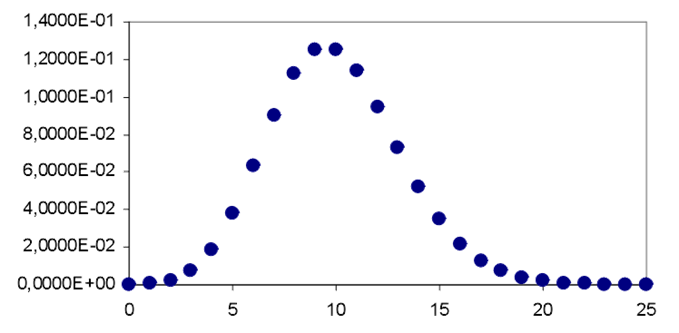
\includegraphics[scale=.5]{ilustraciones/11.png} 
%ilustracion11%
\end{center}
\end{frame}


\begin{frame}{Ejercicio}
Suponga que el número $X$ de tornados observados en una región
particular durante un año tiene una distribución de Poisson con $\lambda=8$.
\bigskip
\begin{enumerate}
  \item Calcule $P(X \le 5)$.
  \item Calcule $P(6 \le X \le 9)$.
  \item Calcule $P(10 \le X)$.
\end{enumerate}

\end{frame}


\section{Resumen}



\begin{frame}{Principales distribuciones de probabilidad discretas}

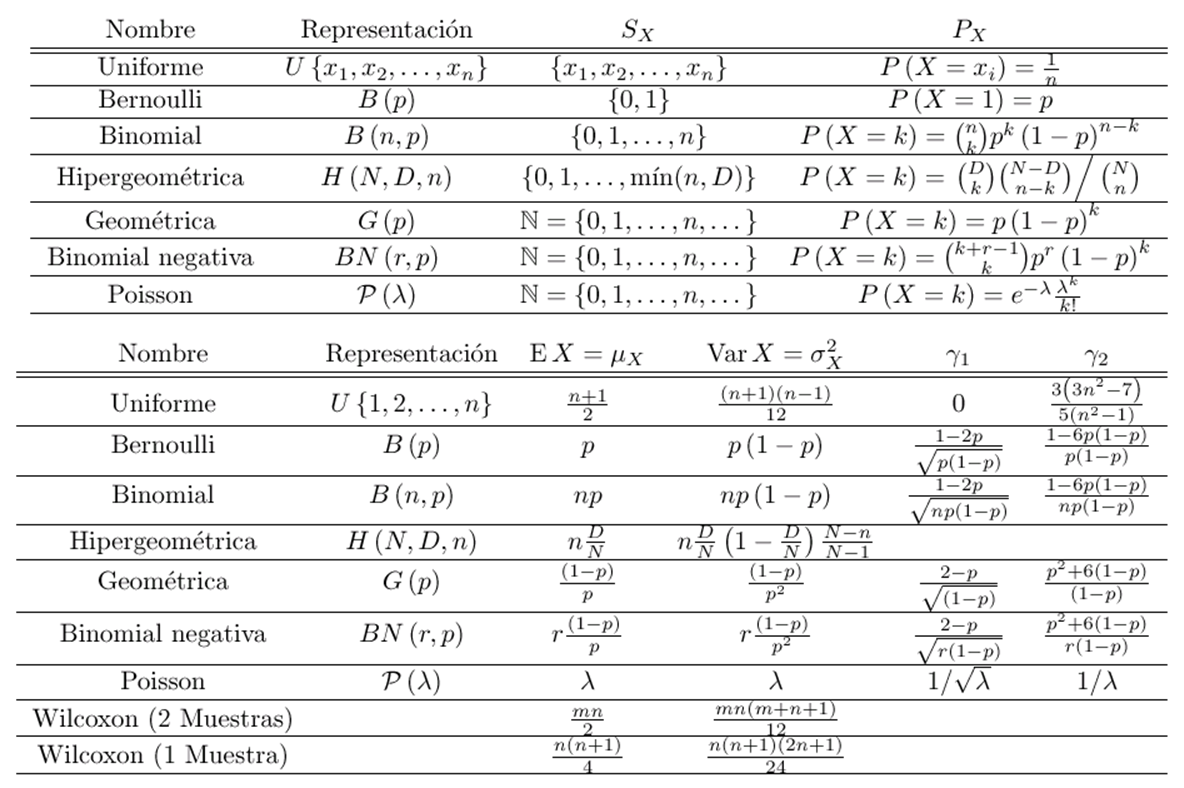
\includegraphics[scale=0.55]{ilustraciones/76.png} 
%ilustracion76%
\end{frame}


\section{Distribuciones discretas conjuntas}
\subsection{Función de probabilidad conjunta}


\begin{frame}{Dos variables aleatorias discretas}
\begin{itemize}
\item
La función de probabilidad de una sola variable aleatoria discreta $X$ especifica cuánta probabilidad está colocada en cada valor posible de $X$.  
\item La función de probabilidad conjunta de dos variables aleatorias discretas $X$ y $Y$ describe cuánta probabilidad se coloca en cada par posible de valores $(x,y)$.
\end{itemize}
\end{frame}


\begin{frame}{}
Sean $X$ y $Y$ dos variables aleatorias discretas  definidas en el espacio muestral $S$ de un experimento. La {\bf función de probabilidad conjunta} $p(x,y)$ se define para cada par de números $(x,y)$ como 
$$p(x,y)=P(X=x,Y=y).$$
Debe cumplirse que $p(x,y) \ge 0$ y $\sum_{x} \sum_{y} p(x,y)=1$.

\bigskip
Ahora sea $A$ cualquier conjunto compuesto por pares de valores $(x,y)$ (por ejemplo, $A= \{(x,y): x+y=5\}$ o $\{(x,y): \max (x,y) \le 3\}$ ). Entonces la probabilidad $P[ (X,Y) \in A]$ se obtiene sumando la función de probabilidad  conjunta incluidos todos los pares en $A$: 
$$P[ (X,Y) \in A] = \sum_{(x,y) \in} \sum_{A} p(x,y)$$
\end{frame}


\begin{frame}{Ejemplo}
Una gran agencia de seguros presta servicios a numerosos clientes que han adquirido tanto
una póliza de propietario de casa como una póliza de automóvil en la agencia. Por cada tipo
de póliza, se debe especificar una cantidad deducible. Para una póliza de automóvil, las
opciones son $\$100$ y $\$250$, mientras que para la póliza de propietario de casa, las opciones
son $\$0$, $\$100$ y $\$200$. Suponga que se selecciona al azar un individuo con ambos tipos de póliza
de los archivos de la agencia. Sea $X=$ la cantidad deducible sobre la póliza de auto y $Y=$ la cantidad deducible sobre la póliza de propietario de casa. Los posibles pares $(X, Y)$ son
entonces $(100, 0)$, $(100, 100)$, $(100, 200)$, $(250, 0)$, $(250, 100)$ y $(250, 200)$; la función 
de probabilidad conjunta especifica la probabilidad asociada con cada uno de estos pares,
con cualquier otro par tiene probabilidad cero.
\end{frame}


\begin{frame}{Ejemplo}

Suponga que la tabla de probabilidad conjunta
siguiente da la función de probabilidad conjunta:
\begin{center}
\begin{tabular}{cc}
& y \\
x &
\begin{tabular}{r|rrr}
p(x,y) & 0 &  100 & 200 \\
\hline 
100 & 0.20 & 0.10 & 0.20 \\
250 & 0.05 & 0.15 & 0.30 
\end{tabular}
\end{tabular}
\end{center}
Entonces $p(100,100)=P(X=100,Y=100)=P(\$100$ deducible sobre ambas pólizas$)=0.10$.

La probabilidad $P(Y \ge 100)$ se calcula sumando las probabilidades de todos los pares $(x,y)$ para los cuales $y\ge100$:
\begin{eqnarray*}
P(Y \ge100)&=&p(100,100)+p(250,100)+p(100,200)+p(250,200) \\
&=& 0.75
\end{eqnarray*}
\end{frame}

\subsection{Función de probabilidad marginal}
\begin{frame}{Función de probabilidad marginal}
La {\bf función de probabilidad marginal} de $X$ y de $Y$, denotadas por $p_X (x)$  y $p_Y (y)$ respectivamente 
$$p_X(x)=P(X=x)=\sum_{y} p(x,y) $$ 
$$ p_Y(y)=P(Y=y)=\sum_{x} p(x,y)$$
\end{frame}


\begin{frame}{Ejemplo}

Para el mismo ejemplo
\begin{center}
\begin{tabular}{cc}
& y \\
x &
\begin{tabular}{r|rrr|r}
p(x,y) & 0 &  100 & 200 & $p_X(x)$ \\
\hline 
100 & 0.20 & 0.10 & 0.20  & 0.50 \\
250 & 0.05 & 0.15 & 0.30 & 0.50 \\
\hline
$p_Y(y)$ & 0.25 & 0.25 & 0.50 & 1.00
\end{tabular}
\end{tabular}
\end{center}


\begin{eqnarray*}
P(Y \ge100)&=&p_Y(100)+p_Y(200) \\
&=& 0.25+0.50\\
&=& 0.75
\end{eqnarray*}
\end{frame}


\begin{frame}{Ejemplo}
La función de probabilidad marginal de $X$ es entonces
$$ p_X(x)=\left\{  \begin{matrix} 0.5 & x=100, 250 \\ 0 & \mbox{de lo contrario} \end{matrix}  \right.$$
Y la función de probabilidad marginal de $Y$ es
$$ p_Y(y)=\left\{  \begin{matrix} 0.25 & y=0, 100 \\ 0.50 & y=200 \\ 0 & \mbox{de lo contrario} \end{matrix}  \right.$$
Por lo tanto $P(Y \ge100)=p_Y(100)+p_Y(200)=0.75$ como habíamos visto.
\end{frame}


\subsection{Variables aleatorias independientes}
\begin{frame}{Variables aleatorias independientes}
En muchas situaciones, la información sobre el valor observado de una de las dos variables $X$ y $Y$ da 
información sobre el valor de la otra variable. En el ejemplo anterior, la probabilidad marginal de $X$ 
con $x = 250$ fue de $0.5$, como lo fue la probabilidad de que $X = 100$. Sin embargo, si se sabe que el 
individuo seleccionado tuvo $Y = 0$, entonces $X = 100$ es cuatro veces más probable que $X = 250$. Por 
lo tanto, existe dependencia entre las dos variables.
\begin{center}
\begin{tabular}{cc}
& y \\
x &
\begin{tabular}{r|rrr|r}
p(x,y) & 0 &  100 & 200 & $p_X(x)$ \\
\hline 
100 & 0.20 & 0.10 & 0.20  & 0.50 \\
250 & 0.05 & 0.15 & 0.30 & 0.50 \\
\hline
$p_Y(y)$ & 0.25 & 0.25 & 0.50 & 1.00
\end{tabular}
\end{tabular}
\end{center}
\end{frame}
\begin{frame}{Variables aleatorias independientes}
En el tema de probabilidad, se señaló que una forma de definir la independencia de dos eventos
es vía la condición de que $P(A \cap B) = P(A) \cdot P(B)$. A continuación se da una definición
análoga de la independencia de dos variables aleatorias.

\bigskip
Se dice que dos variables aleatorias $X$ y $Y$ son {\bf independientes} si por cada par de valores $x$ y $y$,
$$p(x,y)=p_X(x)\cdot p_Y(y) \hspace{30pt} \mbox{cuando }X \mbox{ y }Y\mbox{ son discretas}$$
\end{frame}

\begin{frame}{Ejemplo}
En la situación de la agencia de seguros 
$$p(100,100)=0.10 \ne (0.50)(0.25)=p_X(100)\cdot p_Y(100)$$
de modo que $X$ y $Y$ no son independientes. La independencia de $X$ y $Y$ requiere que toda
entrada en la tabla de probabilidad conjunta sea el producto de las probabilidades marginales que aparecen en la filas y columnas correspondientes.

\end{frame}




\subsection{Función de probabilidad condicional}
\begin{frame}{Función de probabilidad condicional}
En el tema de probabilidad, se señaló que la probabilidad condicional de dos eventos
de define como $P(B \mid A) = P(A \cap B) / P(A)$.  A continuación se da una definición similar para la probabilidad condicional de dos variables aleatorias.

\bigskip 
Sean $X$ y $Y$ dos variables aleatorias discretas con función de probabilidad conjunta $p(x,y)$ y función de probabilidad marginal de $X$ $p_X(x)$. Entonces para  cualquier valor de $x$ de $X$ para el cual $p_X(x)>0$, la {\bf función de probabilidad condicional de $Y$ dado que $X=x$} es
$$p_{Y\mid X}(y\mid x)=\frac{p(x,y)}{p_X(x)} \hspace{30pt} y \mbox{ valor de } Y$$

\end{frame}


\begin{frame}{Ejemplo}

Para el mismo ejemplo $p_{X \mid Y}(x \mid y)$  sería
\begin{center}
\begin{tabular}{cc}
& y \\
x &
\begin{tabular}{r|rrr|r}
$p_{X \mid Y}(x \mid y)$ & 0 &  100 & 200 & $p_X(x)$ \\
\hline 
100 & 0.80 & 0.40 & 0.40  & 0.50 \\
250 & 0.20 & 0.60 & 0.60 & 0.50 \\
\hline
 Total     & 1.00 & 1.00 & 1.00 & 1.00
\end{tabular}
\end{tabular}
\end{center}


$$P_{X \mid Y}(100 \mid Y=0)=0.80$$
\end{frame}


\begin{frame}{Ejemplo}

De manera similar $p_{Y \mid X}(y \mid x)$  es
\begin{center}
\begin{tabular}{cc}
& y \\
x &
\begin{tabular}{r|rrr|r}
$p_{Y \mid X}(y \mid x)$   & 0 &  100 & 200 & Total \\
\hline 
100 & 0.40 & 0.20 & 0.40  & 1.00 \\
250 & 0.10 & 0.30 & 0.60 & 1.00 \\
\hline
 $p_Y(y)$   & 0.25 & 0.25 & 0.50 & 1.00
\end{tabular}
\end{tabular}
\end{center}


$$P_{Y \mid X}(100 \mid X=250)=0.30$$
\end{frame}


\begin{frame}{Propiedades}
A su vez, conociendo la función de probabilidad marginal y condicional, se puede producir la distribución conjunta
\begin{eqnarray*}
p(x,y)&=&p_{X \mid Y}(x\mid y)\cdot p_Y(y) \\
p(x,y)&=&p_{Y \mid X}(y\mid x)\cdot p_X(x) 
\end{eqnarray*}
Las variables aleatorias $X$ y $Y$ serán independientes estadísticamente si las probabilidades condicionales son identicas a las marginales
\begin{eqnarray*}
p_{X \mid Y}(x\mid y) &=&p_X(x) \\
p_{Y \mid X}(y\mid x)&=& p_Y(y) 
\end{eqnarray*}
En el ejemplo planteado, las probabilidades condicionales son diferentes de las marginales y se concluye que las variables están relacionadas.
\end{frame}
\subsection{Ejemplos}

\begin{frame}{Ejemplos}
\begin{enumerate}
\item Se elige un adulto de la ciudad de Aguascalientes y se observa $X=$ peso,  $Y=$ estatura.
\item Se desea medir la concentración de cierto contaminante y existen dos métodos para medirlo. Sea $X=$ la concentración medida con el método 1, $Y=$ la concentración medida con el método 2.
\item Se elige un alumno de nuestro posgrado y se le pregunta $X=$ la calificación de su examen de probabilidad, $Y=$ número de horas por semana que dedicó a estudiar el material.
\item  En una planta automotriz, dos tareas estarán a cargo de robots. La primera consiste en soldar dos bisagras, y la segunda, en apretar tres tornillos. Sea $X=$ el número de soldaduras defectuosas, y $Y=$ el número de tornillos apretados incorrectamente por automóvil producido
\end{enumerate}
\end{frame}


\begin{frame}{Ejemplos (cont.)}
Continuando con el ejemplo de los robots. 

Puesto que $X$ y $Y$ son discretas, $(X,Y )$ es una variable aleatoria discreta bidimensional. Los datos indican que la probabilidad conjunta de $(X, Y )$ en el pasado es la que se muestra en la tabla
\begin{table}[]
\begin{tabular}{|l|l|l|l|l|}
\hline
x\textbackslash{} \textbf{y} & \textbf{0}     & \textbf{1}     & \textbf{2}     & \textbf{3}     \\ \hline
\textbf{0}                  & 0.840 & 0.030 & 0.020 & 0.010 \\ \hline
\textbf{1}                  & 0.060 & 0.010 & 0.008 & 0.002 \\ \hline
\textbf{2}                  & 0.010 & 0.005 & 0.004 & 0.001 \\ \hline
\end{tabular}
\end{table}
\end{frame}


\begin{frame}{Ejemplos (cont.)}
\begin{enumerate}[(a)]
\item ¿Es en verdad una probabilidad conjunta?
\item  Encuentre la distribución marginal de $X$ y de $Y$  
\item Encuentre la distribución marginal acumulada de $X$ y de $Y$ 
\item  Encuentre $E(X)$ , $E(Y)$ 
\item ¿Cuál es la probabilidad  de encontrar a lo más un error (no importa cual defecto sea de los dos)?
\item la probabilidad condicional de $Y$  dado $X=0$ 
\item $P(X>Y)$ 
\item ¿Son independientes $X$ y $Y$? 
\end{enumerate}



\end{frame}



\end{document}

